% EBMA paper for Political Analysis: Full (unblinded) version 
% Written by: Jacob M. Montgomery, Florian Hollenbach, and Michael
% D. Ward.
% Last update on: 15/12/2011
% Last updated : Florian & Mike


%\documentclass[pdftex,12pt,fullpage,oneside,endnotes]{amsart}
\documentclass[12pt,fullpage,endnotes]{article}
%\usepackage{apsr}
\usepackage{array,amsmath,psfrag,amssymb,subfigure,tabularx}
\usepackage{hyperref,multicol}
\usepackage{pa}
\usepackage{booktabs}
\usepackage[usenames]{color}
\usepackage{datetime}
\usepackage{dcolumn}
\usepackage{wrapfig}
\usepackage{setspace}
\usepackage{url}
\usepackage[english]{babel}
\usepackage{times}
\usepackage{multirow}
\usepackage[pdftex]{graphicx}
\usepackage{epstopdf}
\usepackage{lscape}
\usepackage{array}
\usepackage{booktabs}
\usepackage{hyperref}
\usepackage{endnotes}

\newcommand{\note}[1]{\endnote{\doublespacing#1 \vspace{4 mm}}}

\usepackage{natbib}
\bibpunct{(}{)}{;}{a}{}{,}
\bibdata{Bibliography_EBMA}
%\bibliographystyle{chicago}

\newboolean{blind}
\setboolean{blind}{false}


\title{Improving Predictions Using Ensemble \\ Bayesian Model
  Averaging \thanks{For generously sharing their data and models with
    us, we thank Alan Abramowitz, James Campbell, Robert Erikson, Ray
    Fair, Douglas Hibbs, Michael Lewis-Beck, Andrew D. Martin, Kevin
    Quinn, Stephen Shellman, Charles Tien, \& Christopher Wlezien.
    We especially want to thank Adrian Raftery and Brendan Nyhan for their
    encouragement and feedback as this project evolved. The editor and the reviewers of {\em Political Analysis}
    provided especially salient and important suggestions that substantially improved our research.
   This work was supported by the Information Processing Technology Office of the
    Defense Advanced Research Projects Agency through a
    holding grant is to the Lockheed Martin Corporation [FA8650-07-C-7749].}}
\author{
Jacob M. Montgomery\\
	Department of Political Science\\
	Washington University in St. Louis\\
	Campus Box 1063, One Brookings Drive\\
	St. Louis, MO, USA, 63130-4899 
	\and
Florian Hollenbach  \\
	Department of Political Science\\
	Duke University\\
	Perkins Hall 326 Box 90204\\
	Durham, NC, USA, 27707-4330
	\and
Michael D. Ward\\
	Department of Political Science\\
	Duke University\\
	Perkins Hall 326 Box 90204\\
	Durham, NC, USA, 27707-4330\\
	corresponding author: michael.d.ward@duke.edu
} 




\date{\today}


\begin{document}

\maketitle
\thispagestyle{empty}
\clearpage
\pagestyle{myheadings}
\markright{Montgomery, Hollenbach, \& Ward\hfill Ensemble BMA\hfill}
\newpage
\singlespacing

\thispagestyle{empty}


\begin{abstract}
\begin{doublespace}
 We present ensemble Bayesian model averaging (EBMA) and illustrate
  its ability to aid scholars in the social sciences to make more
  accurate forecasts of future events.  In essence, EBMA improves
  prediction by pooling information from multiple forecast models to
  generate ensemble predictions similar to a weighted average of
  component forecasts. The weight assigned to each forecast is
  calibrated via its performance in some validation period. The aim is
  not to choose some ``best'' model, but rather to incorporate the
  insights and knowledge implicit in various forecasting efforts via
  statistical postprocessing.  After presenting the method, we show
  that EBMA increases the accuracy of out-of-sample forecasts relative
  to component models in three applied examples: predicting the
  occurrence of insurgencies around the Pacific Rim, forecasting vote
  shares in U.S. presidential elections, and predicting the votes of
  U.S. Supreme Court Justices.
  \end{doublespace}
\end{abstract}

\doublespacing
\newpage

%%% Insert all of the main text
\setcounter{page}{1}
% Revised by Jacob on Sept 23
% edited by MDW on October 12, 2011
% Revised by Flo on Dec 20, 2011
% edited by Jacob on Dec 20, 2011

\section{Introduction}
Testing systematic predictions about future events against observed
outcomes is generally seen as the most stringent validity check of
statistical and theoretical models.  Yet, political scientists rarely
make predictions about the future.  Empirical models are seldom
applied to out-of-sample data and are even more rarely used to make
predictions about future outcomes. Instead, researchers typically
focus on developing and validating theories that explain past events.

In part, this lack of emphasis on forecasting results from the fact
that it is so difficult to make accurate predictions about complex
social phenomena. However, research in political science could gain
immensely in its policy relevance if predictions were more common and
more accurate.  Improved forecasting of important political events
would make research more germane to policymakers and the general
public who may be less interested in explaining the past than
anticipating and altering the future.  From a scientific standpoint,
greater attention to forecasting would facilitate stringent validation
of theoretical and statistical models since truly causal models should
perform better in out-of-sample forecasting.

In this article, we extend a promising statistical method -- ensemble
Bayesian model averaging (EBMA) -- and introduce software that will
aid researchers across disciplines to make more accurate forecasts.
In essence, EBMA makes more accurate predictions possible by pooling
information from multiple forecast models to generate ensemble
predictions similar to a weighted average of component forecasts. The
weight assigned to each forecast is calibrated via its performance in
some prior period.  These component models can be diverse.  They need
not share covariates, functional forms, or error structures. Indeed,
the components may not even be statistical models, but may be
predictions generated by agent-based models or subject-matter experts.

In the rest of this article we briefly review
existing political science research aimed at forecasting and then
present the mathematical details of the EBMA method. We then
illustrate the benefits of EBMA by applying it to predict insurgency
events on the Pacific Rim, U.S. presidential elections, and voting on
the U.S. Supreme Court.

\section{Dynamic forecasting in political science}
Although forecasting is a rare exercise in political science, there
are an increasing number of exceptions.  In most cases, ``forecasts''
are conceptualized as an exercise in which the predicted values of a
dependent variable are calculated based on a specific statistical
model and then compared with observed values
\citep[e.g.,][]{Hildebrand:etal:1976}. In many instances, this reduces
to an analysis of residuals.  In others, the focus is on randomly
selecting subsets of the data to be excluded during model development
for cross-validation.  However, there is also a more limited tradition
of making true forecasts about events that have not yet occurred.
(See \citet{brandt:freeman:schrodt:2011} for a recent and thorough
survey of forecasts in political science and economics with a focus on
strategies to perform more meticulous comparisons of their accuracy.)


An early proponent of using statistical models to make predictions in
the realm of international relations (IR) was Stephen Andriole
\citep{Andriole:Young:1977}. In 1978, a volume edited by Nazli Choucri
and Thomas Robinson \nocite{Choucri:Robinson:1978} provided an
overview of the then current work in forecasting in IR.  Much of this
work was done in the context of policy-oriented research for the
U.S. government during the Vietnam War.  Subsequently, there were a
variety of efforts to create or evaluate forecasts of international
conflict, including \citet{Freeman:Job:1979},
\citet{Singer:Wallace:1979}, and \citet{Vincent:1980}.  In addition, a
few efforts began to generate forecasts of domestic conflict
\citep[e.g.,][]{Gurr:Lichbach:1986}.  Recent years, however, have
witnessed increasing interest in prediction across a wide array of
contexts in IR.\note{An incomplete list of recent work would include
  \citet{Krause:1997}, \citet{Davies:Gurr:1998},
  \citet{Pevehouse:Goldstein:1999}, \citet{Schrodt:Gerner:2000},
  \citet{King:Zeng:2001}, \citet{OBrien:2002}, \citet{BDM:2002},
  \citet{Fearon:Laitin:2003}, \citet{Demarchi:etal:2004},
  \citet{Enders:Sandler:2005}, \citet{Leblang:Satyanath:2006},
  \ifthenelse{\boolean{blind}}{\citet{Author:2020b}}{\citet{Ward:etal:2007}},
  \citet{Brandt:etal:2008}, \citet{Bennett:Stam:2009}, and
  \ifthenelse{\boolean{blind}}{\citet{Author:2020}}{\citet{Gleditsch:Ward:2010}}. A
  summary of classified efforts is reported in \citet{Feder:2002}.  An
  overview of some of the historical efforts along with a description
  of current thinking about forecasting and decision-support is given
  by \citet{OBrien:2010}.}  The 2011 special issue of \emph{Conflict
  Management and Peace Science} on prediction in the field of IR
exemplifies this growing emphasis on forecasting
\citep[c.f.,][]{Schneider_etal_2011, Mesquita_2011,
  Brandt_etal_2011}. \ifthenelse{\boolean{blind}}{\citet{Author:2020b}}{\citet{wgb:2010}}
and
\ifthenelse{\boolean{blind}}{\citet{Author:2020b}}{\citet{Greenhill:2011}}
provide additional discussion of forecasting in IR.

Outside of IR, forecasting in political science has largely taken
place in the context of election research.  % The most famous election
% prediction was, of course, the prediction of the {\em Chicago Daily
%   Tribune} in 1948 which published incorrect headlines stating that
% Dewey defeated Truman, though as early as 1936 the {\em Literary
%   Digest} falsely predicted the defeat of Roosevelt.
In the 1960s, \citet{Pool:1964} published a volume describing their
work on the 1960 and 1964 presidential elections. They reported their
efforts to use a computer simulation to predict election outcomes,
which was initially undertaken in the context of providing campaign
management advice for the 1960 campaign of John F. Kennedy.
\citet{Rosenstone:1983} published perhaps the most influential early
work on elections forecasting, which surveyed the then state-of-the-art
and included examples going back to 1932.

%  Rosenstone concludes that political scientists were making
% inaccurate forecasts because they did not have a theory of elections.
% The subsequent efforts at predicting elections have mainly focused at
% developing a theory of elections that is based on various factors
% thought to influence turnout and preferences.

In the 1990s, political scientists renewed their interest in
predicting presidential elections \citep{Campbell:1990,
  Campbell:1992}. This work was anticipated by the efforts of several
economists, most notably the forecasts established by Ray C. Fair
(\citeyear{Fair:1978}). As we discuss below, predicting
U.S. presidential and congressional elections has since developed into
a regular exercise.  Moreover, researchers have begun to forecast
election outcomes in France \citep[e.g.,][]{Jerome:1999} and the
United Kingdom
\citep[e.g.,][]{Whitely:2005}.\note{\citet{Lewis-Beck:2005} provides a
  more in-depth discussion of election forecasting in a comparative
  context.} 


While efforts to predict future outcomes remain uncommon, research
that combines multiple forecasts are nearly non-existent.  To our
knowledge, the only non-IR examples are the PollyVote project
\citep[c.f.][]{Graefe:2010}, which combines multiple predictions using
simple averages of forecasts to predict U.S. presidential elections,
and \citet{gelman:forecasts}, who use Bayesian methodology to combine
information from historical state-level election returns, current
polling data, and forecasting models to generate election forecasts.


% from multiple past  
% {\em Political Analysis} that employes a wide range of data, including
% previously collected surveys, estimated uncertainties from the
% surveys, and extant models of electoral politics.  The result shows
% that this approach allows one to use recent data to predict election
% outcomes at the state level, but also showed that less recent surveys
% increases accuracy at the national level. The implication is that
% state-level data can be usefully employed in national level
% predictions via a methodology that uses Bayesian principles to combine
% information.


Yet, combining forecasts, and ensemble methods in particular, have
been shown to substantially reduce prediction error in two important
ways.  First, across subject domains, ensemble predictions are usually
more accurate than any individual component model. Second, they are
significantly less likely to make dramatically incorrect predictions
\citep{Bates:1969, Armstrong:2001, Raftery:2005}.\note{The case for
  using predictions heuristically can also be found in early work by
  \citet{Dawid:1982, Dawid:1984}.}  Combining forecasts not only
reduces reliance on single data sources and methodologies (which
lowers the likelihood of dramatic errors), but also allows for the
incorporation of more information than any one model is likely to
include in isolation.

The idea of ensemble learning itself has a long history in the machine
learning community. The most thorough treatment is found in Hastie,
Tibshirani, and Friedman (2009).  A wide range of statistical
approaches including bagging, random forests, as well as boosting and
penalized methods may be properly considered ensemble approaches. They
are different from EBMA however, which comes from another branch on
the ensemble family tree -- Bayesian statistics.  Bayesian methods
themselves can generally be viewed as ensemble methods, since they
produce a large number of candidate ``models'' that are averaged to
create a posterior distribution of parameters
\citep[p. 605]{Hastie:2009}.

These advances in the statistical literature parallel additional
research in formal theory, which shows that groups of agents using
diverse decision-rules or composed of agents with different viewpoints
on a problem can produce superior outcomes in difficult decision
environments \citep{Page:2007, Page:2008, Page:2011}.  That is, social
systems, organizations, and institutions that are better able to
combine insights and knowledge from diverse actors are more
functional, successful, and adaptive in complex environments.  

This last strain of thought is related to research that suggests the
use of prediction markets as a method of aggregating a large number of
individual predictions about particular events. For example,
\citet{berg:2008} discuss prediction markets and demonstrate that they
can be more accurate than polls when forecasting elections. One
important prediction market in political science is the Iowa
Electronic Market, in which individuals buy futures on politicians
which are paid after election results are revealed.


\section{Ensemble Bayesian model averaging} 

Predictive models remain underutilized, yet an increasing number of
scholars have developed forecasting models for specific research
domains.  As the number of forecasting efforts proliferate, however,
there is a growing benefit from developing methods to pool across
models and methodologies to generate more accurate forecasts.  Very
often, specific predictive models prove to be correct only for certain
subsets of observations.  Moreover, specific models tend to be more
sensitive to unusual events or particular data issues than ensemble
methods.

To aid the newfound emphasis on prediction in political science, we
are advancing recent statistical research aimed at integrating
multiple predictions into a single improved forecast.  In particular,
we are adapting an ensemble method first developed for application to
the most mature prediction models in existence -- weather forecasting
models.  To generate predictive distributions of outcomes (e.g.,
temperature), weather researchers apply ensemble methods to forecasts
generated from multiple models \citep{Raftery:2005}.  Thus,
state-of-the-art ensemble forecasts aggregate multiple runs of (often
multiple) weather prediction models into a single unified forecast.

The particular ensemble method we are extending for application to
political outcomes is ensemble Bayesian model averaging (EBMA). First
proposed by \citet{Raftery:2005}, EBMA pools across various forecasts
while meaningfully incorporating \textit{a priori} uncertainty about
the ``best'' model.  It assumes that no particular model or
forecasting method can fully encapsulate the true data-generating
process.  Rather, various research teams or statistical techniques
will reflect different facets of reality. EBMA collects \textit{all}
of the insights from multiple forecasting efforts in a coherent
manner.  The aim is not to choose some ``best'' model, but rather to
incorporate the insights and knowledge implicit in various forecasting
efforts via statistical post-processing.  In recent years, variants of
the EBMA method have been applied to subjects as diverse as inflation
\citep{Wright:2009, Koop:2010, Gneiting:2010}, stock prices
\citep{Billio:2011}, economic growth and policymaking
\citep{Brock:2007, Billio:2010}, exchange rates \citep{Wright:2008},
industrial production \citep{Feldkircher:2010}, ice formation
\citep{Berrocal:2010}, visibility \citep{Chmielecki:2010}, water
catchment streamflow \citep{Viney:2009}, climatology \citep{Min:2006,
  Min:2007, Smith:2009}, and hydrology \citep{Zhang:2009}.  Indeed,
research is underway to extend the method to handle missing data
\citep{Fraley:2010, Mccandless:2011} as well as calibrate model
weights on non-likelihood criteria \citep[e.g.,][]{Vrugt:2006}.



\subsection{Overview of method}

EBMA is designed for application in the context of a subject-domain
with ongoing forecasting efforts.  That is, it assumes the existence
of multiple teams or individuals making regular predictions about a
common set of outcomes.  For example, there may be multiple analysts
or teams making predictions about the likelihood of violent conflict
in specific regions of the world, quarterly economic growth for the
United States, or the votes of members on bills before Congress.  As
we show in our examples below, these predictions might originate from
the insights and intuitions of individual subject-experts, traditional
statistical models, non-linear classification trees, neural networks,
agent based models, or anything in between. 

EBMA is a method for taking the predictions made by multiple teams and
combining them -- based on their past performance and uniqueness -- to
create a new ensemble forecasting model.  This ensemble model can then
make predictions about unobserved outcomes in the future and usually
outperforms its components.  Roughly speaking, it creates forecasts by
creating weighted averages of component predictions, or component
predictive probability distribution functions (PDFs).  The weight
assigned to each component forecast, denoted $w_k$ below, reflects two
aspects of the components' past forecasts.  First, \textit{ceteris
  paribus}, the EBMA model will give greater weight to forecasts that
were more accurate in the past.  Second, \textit{ceteris paribus}, it
will assign a greater weight to models that made unique (but correct)
predictions.  That is, component forecasts that are too highly
correlated may jointly have a large weight, but will individually be
penalized.


There are two important aspects of EBMA that distinguish it from the
alternative model-selection or averaging methods referenced above.
First, EBMA is more flexible in not requiring any information about
the actual covariates that go into the component models. A second, and
related point is that EBMA does not require researchers to develop
metrics to penalize component forecasts for the number of parameters
included, the number of covariates, or their complexity more
generally.  In the case of subject-expert opinions, there may not even
be any covariates or statistical models involved, a point we return to
in the Supreme Court example below. Another non-statistical component
model that researchers might include is prices on prediction markets.
In other instances, predictions may come from models whose
``complexity'' is not easily defined or enumerated (e.g., agent-based
models).  Of course, overly-complex ``garbage can'' models will
generally perform poorly when making predictions over any outcome and
therefore receive a lower weight in the ensemble forecast.  Yet, this
lower weight is a function of the model's predictive performance
rather than a pre-specified preference for parsimony.  The upshot is
that EBMA forecasts will implicitly penalize over-fitting of component
models since the weight assigned to component models is based on
predictive performance.  However, it can do so without explicitly
penalizing components for complexity.\note{To fully capture the
  ability of EBMA to reduce over-fitting when using statistical models
  it is necessary to divide the data into three periods
  \citep{Hastie:2009}.  The first period, the training period, is used
  to fit the parameters for each component model.  The second period,
  the validation period, is used to calculate model weights and other
  parameters for the EBMA model using out-of-sample predictions
  generated from the component models.  We then generate ensemble
  predictions for the third period, the test period, using the EBMA
  model parameters calculated in period two.  This approach is
  explicit in the insurgency forecasting example below and implicit in
  the Supreme Court example below since the subject-experts and
  classification algorithm were ``trained'' on data not included in
  the study. This three-stage method is adjusted in the election
  forecasting example as the component models are already sparse
  (somewhat ameliorating concerns about over-fitting) and there are a
  much smaller number of observations.  In this example, component
  models are trained over the period beginning in 1916 and the EBMA
  parameters are calculated only for the period beginning in 1952.
  However, there is significant overlap in the training and validation
  samples. \label{samples}}



\subsection{Mathematical foundations}

EBMA itself is an extension of the Bayesian model averaging (BMA)
methodology \citep[c.f.,][]{Madigan:1994, Draper:1995, Raftery:1995,
  Hoeting:1999, Clyde:2003, Raftery:2003, Clyde:2004} that has
received considerable attention in the field of statistics. BMA was
first introduced to political science by \citet{Bartels:1997} and has
been applied in a number of contexts \citep[e.g.,][]{Bartels:2001,
  Gill:2004, Imai:2004,
  Geer:2006b}. \ifthenelse{\boolean{blind}}{\citet{Author:2020b}}{\citet{Montgomery:2010c}}
provide a more in-depth discussion of BMA and its applications in
political science.


Assume we have some quantity of interest to forecast,
$\mathbf{y}^{t^*}$, in some future period $t^\ast \in
T^\ast$.  Further assume that we have extant forecasts for events
$\mathbf{y}^t$ for some past period $t \in T$ that were generated from
$K$ forecasting models or teams, $M_1, M_2, \ldots, M_K$. Each model,
$M_k$, is assumed to come from the prior probability distribution
$M_k\sim \pi(M_k)$, and the PDF for $\mathbf{y}^t$ is
$p(\mathbf{y}^t|M_k)$. The outcome of interest is distributed
$p(\mathbf{y}^{t^*}|M_k$).  Applying Bayes Rule, we get that
\begin{equation} \small
p(M_k|\mathbf{y}^t) = \frac{p(\mathbf{y}^t|M_k)\pi(M_k)}{\underset{k=1}{\overset{K}{\sum}}p(\mathbf{y}^t|M_k)\pi(M_k)}
\end{equation}
\noindent and the marginal predictive PDF is
\begin{equation}
\label{BMA-pdf}
\small
p(\mathbf{y}^{t^*}) = \underset{k=1}{\overset{K}{\sum}} p(\mathbf{y}^{t^*}|M_k)p(M_k|\mathbf{y}^{t}).
\end{equation}
The BMA PDF (\ref{BMA-pdf}) can be viewed as the weighted average of
the component PDFs where the weights are determined by each model's
performance within the already-observed period $T$.  Likewise, we can
simply make a deterministic estimate using the weighted predictions of
the components, denoted
%\begin{equation} \small
$E(\mathbf{y}^{t^*}) = \underset{k=1}{\overset{K}{\sum}}
E(\mathbf{y}^{t^*}|M_k)p(M_k|\mathbf{y}^{t})$. 
%\end{equation}

\subsubsection{EBMA for dynamic settings: }

In generating predictions of future events, the task is to first build
a set of statistical models for some set of observations $S$ in the
past time periods $T^{\prime}$, which we refer to as the training
period.  Using these models, we then generate predictions
$\mathbf{f}^{s|t}_k$ for some period $T$, which has already occurred
but which was not included in the training sample.  We refer to this
as the validation period, and we will use this data to calibrate the
EBMA model.\note{In the case of subject-experts, the training period
  is implicitly the period over which experts have gained their
  experience.  Forecasts will only be necessary for the validation
  period.}  Finally, using the same $K$ models, we assume that there
are true forecasts ($\mathbf{f}_k^{s|t^\ast}$) for observations $s \in
S$ in future time periods $t^\ast \in
T^*$.\note{\citet{Sloughter:2007} make predictions for only one future
  time period, and use only a subset of past time-periods (they
  recommend 30) in their validation period. Thus, predictions are made
  sequentially with the entire EBMA procedure being re-calculated for
  each future event as observations are moved from the test period
  $T^\ast$ into the validation period $T$. Another alternative is to
  simply divide \textit{all} the data into discrete training, validation and
  test periods for the entire procedure.  We use both approaches in
  our examples below.}  We either (a) treat these raw predictions as a
component model in the steps below or (b) statistically post-process
the predictions for out-of-sample bias reduction and treat these
re-calibrated predictions as a component model.

As a running example, let us assume that we have $K$ forecasting
efforts for modeling insurgencies in a set of countries $S$ ongoing
throughout the training ($T^{\prime}$) validation ($T$) and test
($T^\ast$) periods.  We will associate each component forecast with a
component PDF, $g_k(\mathbf{y}|\mathbf{f}_k^{s|t, t^\ast})$, which may
be the original prediction from the forecast model or the
bias-corrected forecast.


The EBMA PDF is then a finite mixture of the $K$ component PDFs,
denoted
\begin{equation}
\small
\label{BMA-eq}
p(\mathbf{y}|\mathbf{f}_1^{s|t}, \ldots, \mathbf{f}_K^{s|t})=\overset{K}{\underset{k=1}{\sum}} w_k
g_k(\mathbf{y}|\mathbf{f}_k^{s|t}),
\end{equation}
\noindent The $w_k$'s $\in [0,1]$ are model probabilities and
$\sum_{k=1}^Kw_k=1$.  Roughly speaking, they are associated with each
component model's predictive performance in the validation period
controlling for the degree to which they offer unique insight (i.e.,
a model's predictions are distinct from those of other component models).
We provide additional discussion about the model weights in the
election forecasting example below.  Details for parameter estimation
are provided in Appendix A.  The ensemble PDF for an insurgency in the
test period $t^\ast$ in country $s$ is then:
\begin{equation}
\label{BMA-eq2}
\small
p(y|f_{1}^{s|t^\ast}, \ldots,
f_{K}^{s|t^\ast})=\overset{K}{\underset{k=1}{\sum}} w_k
g_k(y|f_{k}^{s|t^*}).
\end{equation}


\subsubsection{EBMA for normally distributed outcomes:}
To gain a fuller understanding of the EBMA method, it is easiest to
imagine an effort to predict some normally distributed outcome.  When
forecasting outcomes that are distributed normally,
\citet{Raftery:2005} propose approximating the conditional PDF as a
normal distribution centered at a linear transformation of the
individual forecast, $g_k(\mathbf{y}|\mathbf{f}_k^{s|t}) = N(a_{k0} +
a_{k1}\mathbf{f}_k^{s|t}, \sigma^2)$.  Prior applications have found
that this adjustment of the component models' forecasts reduces
over-fitting and improves the performance of the final ensemble
forecasting model \citep{Raftery:2005}.\note{Our adjustments to the
  basic EBMA method for application to dichotomous outcomes, as well
  as details of parameter estimation, are shown in Appendix A.}  Using
\eqref{BMA-eq} and \eqref{BMA-eq2} above, the EBMA PDF is then
\begin{equation} \small
p(\mathbf{y}|\mathbf{f}_1^{s|t}, \ldots, \mathbf{f}_K^{s|t}) = \overset{K}{\underset{k=1}{\sum}} w_k N(a_{k0} +
a_{k1}\mathbf{f}_k^{s|t}, \sigma^2),
\end{equation}
\noindent and the predictive distribution for some observation $y$ is 
\begin{equation} \small
p(y|f_1^{s|t^\ast}, \ldots, f_K^{s|t^\ast}) = \overset{K}{\underset{k=1}{\sum}} w_k N(a_{k0} +
a_{k1}f_k^{s|t^\ast}, \sigma^2)
 \end{equation}
 \noindent Thus, the predictive PDF is a mixture of $K$ normal
 distributions each of whose mean is determined by the component
 prediction ($f_k^{s|t^\ast}$) and whose ``height'' (i.e, the total
 area under the curve for component $k$) is determined by the model
 weight $w_k$.




\section{Empirical applications}

In this section, we provide empirical applications of EBMA to predict
insurgency in the Pacific Rim, presidential election outcomes in the
United States, and votes of Justices of the United States Supreme
Court.  These three examples demonstrate the usefulness of the method
for diverse domains of political science research, different types of
outcomes of interest (i.e., dichotomous and continuous), and different
forms of component models (i.e., statistical models versus expert
predictions).



\subsection{Application to insurgency forecasting}

Our first example applies the EBMA method to data collected for the
Integrated Crisis Early Warning Systems (ICEWS) project sponsored by
the Defense Advanced Research Projects Agency (DARPA).  The task of
the ICEWS project is to train models on data (focusing on five
outcomes of interest) for 29 countries for every month from 1997
through the present and to then make accurate predictions about
expected crisis events.\note{The twenty-nine countries are Australia,
  Bangladesh, Bhutan, Cambodia, China, Comoros, Fiji, India,
  Indonesia, Japan, Laos, Madagascar, Malaysia, Mauritius, Mongolia,
  Myanmar, Nepal, New Zealand, North Korea, Papua New Guinea,
  Philippines, Russia, Singapore, Solomon Islands, South Korea, Sri
  Lanka, Taiwan, Thailand, and Vietnam. This set is not a random
  sample, but rather constitutes the countries of population greater
  than $500,000$ that are in the area of responsibility of the US
  Pacific Command.}  For purposes of demonstration, we focus on only
one of these outcomes -- violent insurgency.

The bulk of the data for the ICEWS project is gleaned from natural
language processing of a continuously updated harvest of news stories
(primarily taken from Lexus/Nexus and Factiva archives). These are
digested with a version of the TABARI processor for events developed
by Philip Schrodt and colleagues in the context of the Event Data
Project (see \url{http://eventdata.psu.edu/} for more details).  These
data are augmented with a variety of covariates including:
country-level attributes (coded on a monthly or yearly basis) from the
Polity and World Bank datasets, information about election cycles (if
any), events in neighboring countries, and the length of shared
borders with neighboring countries.

\subsubsection{Component models:}

We apply EBMA to make predictions for the occurrence of insurgency in
these 29 countries for each month in the year 2010 (the last year in
the dataset). As a first step in the process, we must choose some set
of observations that we wish to treat as a training period for the
component statistical models and a second set of data to treat as a
validation set with which to calibrate the EBMA model.

Unfortunately, there is no clear guidance available on how to choose
the relative sizes of the training set, the validation set, or the
test set.  Hastie, Tibshirani, and Friedman (2009, Chpt. 7) discuss
this in some detail, wherein they note (p. 195): ``It is difficult to
give a general rule on how to choose the number of observations in
each of the ... parts, as this depends on the signal-to-noise ratio in
the data and the training sample size.''  The basic point is that there is
no general rule. Moreover, the appropriate size of training and test set
depends on the prevalence of the signal in the training data. In the
case of predictive studies like ours, the only general rule is: it
depends.  % In some sense the precision and accuracy of the resultant
% predictions may show that the training set is large enough, but poor
% performance could also indicate that the signal in the data was too
% weak to be discerned.

In this case, we estimated three exemplar statistical models using
data for the \textit{training period} ranging from January
1999\note{Because some of the models include lagged data, this is the
  first year for which all of the component models produce fitted values or predictions.} to
December 2007, and fit an EBMA model using the component model
predictions for the \textit{validation period} ranging from January
2008 to December 2009.  We then make forecasts for the \textit{test
  period} ranging from January 2010 to December 2010 using both the
component and EBMA models.  To provide variation in the complexity (as
well as accuracy) of the components, we included the following models.

%%%%% THOUGHT: We could include a table here listing the training,
%%%%% validation, test periods

\begin{list}{\labelitemi}{\leftmargin=1em}
\item \textbf{SAE}: This is one model developed as part of the ICEWS
  project and was designed by Strategic Analysis Enterprises. It is
  specified as a simple generalized linear logistic model including 27
  different independent variables.\note{See
    \url{strategicanalysisenterprises.com} for more details.  All data
    and models will be included in a replication dataset at the time
    of publication.}  All of the variables are taken from the ICEWS
  event-stream data.
\item \textbf{GLM}: For the purposes of demonstrating the properties
  of the EBMA method, we estimated a crude logistic model that
  includes only \textit{population size}, \textit{GDP growth} (both
  lagged three months), the number of \textit{minority groups at risk} in the country,
  and a measure of \textit{anocracy} supplied in the \textit{Polity IV} dataset
  \citep{PolityIV}.
\item \textbf{LMER}: This is a generalized linear mixed effects model
  using a logistic link function and including a random effects term
  for lagged \textit{GDP per capita} and the lagged number of
  \textit{conflictual events involving the United states} in the
  country of interest.\note{It is worth noting that the mixed effects model is a kind of 
  ensemble mixture in that in averages the so-called within model with the between model.} The list of additional covariates includes: the
  number of \textit{conflictual events involving the military} within
  the country of interest (lagged three months), the number of
  \textit{days elapsed since the last election},\note{This is
    calculated as the number of days between the middle of the current
    month and the last federal election regardless of the legitimacy
    of the election.} the number of \textit{new insurgencies} that
  began in the previous two years, and a \textit{spatial lag} that
  reflects recent occurrences of domestic crises in the countries'
  geographic neighbors.\note{Geographical proximity is measured in
    terms of the length of the shared border between the two
    countries.}
\end{list}


\subsubsection{Results:}



Table \ref{InSam1} shows the EBMA model parameters as well as fit
statistics associated with the individual component models and the
EBMA predictions for the validation time period (2008-2009). The first
column shows the weights that the EBMA model assigned to each
component. As can be seen, the GLM model is effectively excluded,
while the LMER model carries the greatest weight ($w_k=0.85$)
followed by the SAE model ($w_k = 0.14$).  The constant term
associated with each component corresponds to the term $a_{k0}$ in
(\ref{one}), while the predictor corresponds to $a_{k1}$.  The other
columns in Table \ref{InSam1} are fit statistics.  AUC is the area
under the Receiver-Operating Characteristic (ROC) curve. The advantage
of using ROC curves is that it evaluates forecasts in a way that is
less dependent on an arbitrary cutoff point.  A value of 1 would mean
that all observations were predicted correctly at all possible cutoff
points \citep{King:Zeng:2001}.

\marginpar{\bf{Table \ref{InSam1} about here}}
  
We compare the models using three additional metrics.  The
proportional reduction in error (PRE) is the percentage increase of
correctly predicted observations relative to some pre-defined base
model. In this case, the base model is predicting ``no insurgencies''
for all observations.  Insurgencies are relatively rare events.  Thus,
predicting a zero for all observations leads to a 91.8\% correct
prediction rate. The Brier score is the average squared deviation of
the predicted probability from the true event (0 or 1).  Thus, a lower
score corresponds to higher forecast accuracy \citep{Brier:1950}.
Finally, we calculate the percentage of observations that each model
would predict correctly using a 0.5 threshold on the predicted
probability scale.

\marginpar{\bf{Figure \ref{InSam1sep} about here}}

Note that the EBMA model does at least as well (and usually better)
than all of the component models on almost all of our model fit statistics.
The EBMA model has the highest PRE and \% correct and the lowest Brier
score.  Although the LMER model has a slightly higher AUC, that
model's overall performance suggests that it may be over-fit.


Figure \ref{InSam1sep} shows separation plots for the EBMA model and
the individual components \citep{Greenhill:2011}. In each plot, the
observations are ordered from left to right by increasing predicted
probabilities of insurgency (as predicted by the particular
model). The black line corresponds to the predicted probability
produced by the relevant model for each observation and actual
occurrences of insurgencies are colored red.  Figure \ref{InSam1sep}
shows visually that the GLM model performs very poorly, whereas the
LMER model performs very well, but tends to assign high probabilities
to a large number of observations where we observe no insurgencies
(i.e., it over-predicts insurgencies).  More importantly, the overall
best performance is associated with the EBMA forecast. The separation
plots show that the EBMA model produces few false negatives and
significantly fewer false positives than any of the component models.


However, the more interesting evaluation of the EBMA method is its
test-period predictive power. Table \ref{OutSam1} shows fit statistics
for the individual components as well as the EBMA forecasts for
observations in the 12 months following the validation period.  The
EBMA model outperforms the component models on all metrics.  In
particular, the EBMA model has the highest PRE at 0.43.  Since it is
possible to predict 89.9\% of these observations correctly by
forecasting ``no insurgency,'' a 43\% reduction of error relative to
the baseline model is quite substantial.

\marginpar{\bf{Table \ref{OutSam1} about here}}


Importantly, EBMA clearly outperforms all component models in regard
to the Brier score. Research regarding scoring rules for forecasts has
shown that the Brier score is one of the best statistically proper
scoring rules for evaluating predictions of binary dependent variables
\citep{Gneiting_Raftery_2007}.  Thus, to generally compare and rank
the different models one should use the Brier score
\citep{Gneiting_Raftery_2007}. As can be seen in Tables \ref{InSam1}
and \ref{OutSam1}, the EBMA model has the lowest Brier score in both
the validation and test-period forecasts.\note{One alternative
  approach to generating ensemble forecasts would be to use the simple
  average of each component forecast.  However, this causes
  difficulties because the researcher must use their own judgement to
  decide which alternative models are sufficiently accurate and
  diverse for inclusion.  EBMA offers a more statistically motivated
  and straightforward method for achieving the same end.  In any
  case, these simple averages do not perform well against the EBMA
  forecast.  In the current example, a simple unweighted average
  results in $AUC = 0.885$, PRE=0.123, Brier = 0.052, and \% Correct =
  $92.8$ for the test-period.  This is not surprising given that simple
  averaging weights an inaccurate model the same as an accurate
  one. EBMA on the other hand is able to detect the superiority of
  components and calibrates weights accordingly.  Likewise, simple
  averages cannot identify pairs or groups of highly correlated
  forecasts and will tend to give these groupings too much weight.}

Figure \ref{OutSam1sep} shows the separation plots for the components
as well as the EBMA forecasts for 2010.  The EBMA model again performs
better than any of the individual components with very high predicted
probabilities for the majority of actual events without
over-predicting too many events.  Taking both the fit statistics and
the visual evidence together, we can conclude that the EBMA model
leads to a substantial improvement in test-period forecasts relative
to its components.  This is true even in datasets with rare events and
even when the individual components are already performing well.

\marginpar{\bf{Figure \ref{OutSam1sep} about here}}

\subsection{Application to US presidential election forecasts}
For the past several U.S. election cycles, a number of research teams
have developed forecasting models and published their predictions in
advance of Election Day.  For example, before the 2008 election, a
symposium of forecasts was published in \emph{PS: Political Science
  and Politics} with forecasts of presidential and congressional vote
shares developed by \citet{Campbell:2008}, \citet{Norpoth:2008},
\citet{Lewis-Beck:Tien:2008}, \citet{Abramowitz:2008},
\citet{Erikson:Wlezien:2008}, \citet{Holbrook:2008},
\citet{Lockerbie:2008} and \citet{Cuzan:Bundrick:2008}.  Responses to
the forecasts were published in a subsequent issue. Earlier, in 1999,
an entire issue of the \textit{International Journal of Forecasting}
was dedicated to the task of predicting presidential elections
\citep{Brown:1999}.  Predicting presidential elections has also drawn
the attention of economists seeking to understand the relationship
between economic fundamentals and political outcomes.  Two prominent
examples include work by Ray Fair (\citeyear{Fair:2010}) and Douglas
Hibbs (\citeyear{Hibbs:2000}).

\subsubsection{Component models:}

In the rest of this subsection, we replicate several of these models
and demonstrate the usefulness of the EBMA methodology for improving
the prediction of single important events.\note{It is important to
  note that we attempted to replicate each of the models for the 2008
  election as closely as possible given the model descriptions in the
  articles and the data provided by the authors. We then proceeded to
  use the same model specifications as used in the 2008 articles to
  forecast all elections previous to 2008. Thus, prior to 2008 the
  individual model results are not exact replications of the author's
  given prediction for that election year and results may vary from
  what was presented by the authors as the forecast for a given
  election. This may be due to changes in the model specification over
  time and data updates.  Thus, we neither attempted nor succeeded in
  replicating the exact forecasts for all election years for all
  components.}  We include forecasting models from six of the most
widely cited presidential forecasting teams.  Note that we do not, in
every case, replicate the particular model which the authors identify
as their definitive forecast.
\begin{list}{\labelitemi}{\leftmargin=1em}
\item \textbf{Campbell}: Campbell's ``Trial-Heat and Economy Model''
  \citep{Campbell:2008}
\item \textbf{Abramowitz}: The ``Time-for-Change Model'' created by   \citet{Abramowitz:2008}
\item \textbf{Hibbs}: Hibbs' ``Bread and Peace Model'' \citep{Hibbs:2000}
\item \textbf{Fair}: Fair's presidential vote-share model\note{The model here replicates Equation 1 in \citet{Fair:2010}.}
\item \textbf{Lewis-Beck/Tien}: Lewis-Beck and Tien's ``Jobs Model Forecast'' \citep{Lewis-Beck:Tien:2008}
\item \textbf{EWT2C2}: Column 2 from Table 2 in \citet{Erikson:Wlezien:2008} 


\end{list}
\noindent With the exception of the Hibbs forecast, the models are
simple linear regressions. The dependent variable is the share of the
two-party vote received by the incumbent-party candidate.\note{The
  data to replicate the models by \citet{Abramowitz:2008},
  \citet{Campbell:2008}, \citet{Erikson:Wlezien:2008}, and
  \citet{Lewis-Beck:Tien:2008} were provided in personal
  correspondence with the respective authors.  The remaining data were
  downloaded from the web sites of Ray C. Fair \nocite{Fair2011} (\url{http://fairmodel.econ.yale.edu/vote2012/tbl1.txt}) and
  Douglas Hibbs \nocite{Hibbs2011} (\url{http://www.douglas-hibbs.com/}).}


\subsubsection{Results:}

Rather than selecting a single partition of the data into training,
validation, and test periods (as in the insurgency analysis) we
generate sequential predictions.  For each year from 1976 to 2008, we
use all available prior data to fit the component models.\note{For
  example, the Fair model uses data for election results beginning in
  1916 while the Abramowitz model begins with data from the 1952
  election. }  We then fit the EBMA model using the components'
performances for election years beginning with 1952 (the year when all
models begin generating predictions).  For example, to generate
predictions for the 1988 election, we used the performance of each
component for the 1952-1984 period to estimate model weights.\note{See
  footnote \ref{samples} for additional discussion of the implications
  of the overlapping training and validation samples.  Results in this
  section were computed using modifications of the `ensembleBMA'
  package \citep{Fraley:2010b, Fraley:Forthcoming}.  Because of the
  paucity of data, we did not apply any bias correction to these
  forecasts.  Thus, the predictor and constant, denoted $a_{0k}$ and
  $a_{1k}$ above, are constrained to zero and one respectively.}



\marginpar{\bf{Table \ref{Pres-Year-Res} about here}}

 Table \ref{Pres-Year-Res} provides exemplar results for the 2004 and
 2008 elections.  Table \ref{Pres-Year-Res} shows the weights assigned
 to each model as well as the validation-period root mean squared
 error (RMSE) and mean absolute error (MAE) for the components and the
 EBMA forecasts.\note{As we noted above, these models are fit
   sequentially, so the validation periods change.  For example, the
   validation period for the forecast of the 2004 election is
   1952-2000.  The validation-period RMSE is therefore calculated for
   those observations.  For the 2008 election, the validation period
   is 1952-2004.\label{clarity}} Table \ref{Pres-Year-Res} also shows
 the prediction errors, calculated as the difference between predicted
 and actual values in each year for each component model and the EBMA
 forecast.

 The example results in Table \ref{Pres-Year-Res} illustrate three
 important points.  First, the EBMA model does better than any
 individual component on validation-sample measures of model fit such
 as RMSE and MAE (see Footnote \ref{clarity}).  Second, these results
 demonstrate that EBMA is not guaranteed to generate the most accurate
 prediction for any single observation.  In each year, at least one
 component model comes closer to predicting the actual outcome.
 However, the EBMA forecasts will very rarely provide egregiously
 wrong predictions (e.g., as found in the Campbell model in 2008 and
 the Fair model in 2004) since it borrows strength from multiple
 components.  Moreover, as we show below, in the aggregate the EBMA
 model tends to provide the best forecast over time.

 Third, Table \ref{Pres-Year-Res} shows that there is no clean a
 relationship between validation-sample model performance and model
 weights. For instance, the weight for the Abramowitz model in 2008 is
 $0.001$ even though it has the lowest RMSE and MAE of any component.
 The diminished relationship between validation-sample performance and
 weight is a result of high correlations between forecasts.\note{The
   correlation matrix between fitted-values of the
   model for the 1952-2004 period is: \\

\begin{tabular}{l  rrrrrr}
  \toprule
 & \textbf{C}& \textbf{A} & \textbf{H}& \textbf{F} & \textbf{L} & \textbf{E} \\ 
  \midrule
\textbf{C}ampbell& 1.00 &  &  &  &  & \\
\textbf{A}bramowitz & 0.94 & 1.00 &  &  &  & \\
\textbf{H}ibbs & 0.91 & 0.93 & 1.00&  &  & \\
\textbf{F}air & 0.87 & 0.89 & 0.89 & 1.00&  & \\
\textbf{L}ewis-Beck/Tien & 0.93 & 0.96 & 0.91 & 0.88 & 1.00 & \\
\textbf{E}WT2C2 & 0.85 & 0.90 & 0.87 & 0.91 & 0.86 & 1.00\\
   \bottomrule
 \end{tabular}.}
For instance, fitted values for the Abramowitz model are correlated at
$0.94$ with the Campbell model and at $0.96$ with the Lewis-Beck/Tien
model. Thus, conditioned on knowing these forecasts, the Abramowitz
component provides limited additional information.  

In general, as the number of models included as EBMA components
increases, the risk of including highly correlated forecasts will also
rise.  Researchers should be aware of the fact that adding additional
forecasts as components will not necessarily improve the performance
of EBMA.  EBMA performance will instead be improved by the inclusion
of increasing numbers of \textit{diverse} and \textit{accurate}
forecasts \citep[see also,][]{Graefe:2010}.  Including a large number
of extremely correlated forecasts may actually reduce the benefits of
ensemble forecasting.  However, we note that in practice this is
unlikely to be a significant concern as there are few domains in
political science for which there are large numbers of ongoing
forecasting efforts.


With the 2004 and 2008 examples in mind, we now turn to the relative
test-sample performance of the EBMA and component forecasts across the
entire 1976-2008 period.  Table \ref{Pres-Res} shows the test-sample
RMSE and MAE statistics as well as the percentage of observations that
fall within the 67\% and 90\% predictive intervals for each model.  For our
purposes here, the main result in Table \ref{Pres-Res} is that the
EBMA model again outperforms all components.  The first two columns
show this to be true in terms of predicted error (RMSE and
MAE).\note{\citet{brandt:freeman:schrodt:2011} survey a variety of
  metrics in addition to those we employ here. These include measures
  of average prediction errors, measures using medians and geometric
  averages, measures that compare the complete difference in
  probability distributions, and sequential rank-based methods.
  Although there are many candidate metrics, at least for the
  alternative metrics we have calculated so far, the substantive
  conclusions we reach do not change for our examples and they are not
  presented due to space constraints.  However, as suggested by a
  helpful reviewer, we note that there are reasons to doubt that RMSE
  or MAE will necessarily provide a ranking of component models based
  on accuracy.  A more complete approach evaluating the accuracy of
  the component models is to examine the results displayed in Figure
  \ref{PresPlots2} below.}

\marginpar{\bf{Table \ref{Pres-Res} about here}}

\marginpar{\bf{Figure \ref{PresPlots2} about here}}

 In addition, the coverage statistics demonstrate better calibration
 of EBMA forecasts relative to its component models.  For instance,
 the observed outcome falls within the 67\% predictive interval for
 the Abramowitz model only three out of nine times, while it covers the
 observed values eight out of nine times for the Lewis-Beck/Tien
 model.  Meanwhile, the EBMA 90\% and 67\% predictive intervals are
 nearly perfectly calibrated.

 In a well-calibrated forecasting model, out-of-sample outcomes should
 fall within predictive intervals at a rate corresponding to their
 size.  For instance, the goal is for two-thirds of all out-of-sample
 observations to fall within their respective 67\% predictive
 intervals.  Poorly calibrated models will tend to produce predictive
 intervals that are either too narrow, generating inaccurate
 predictions, or too large, generating predictions that are accurate
 but too vague to be useful.  The better calibration of the EBMA model
 can be seen visually in Figure \ref{PresPlots2}.  The plot shows the
 point predictions and the 67\% and 90\% predictive intervals for each
 model in each year.  The vertical dashed lines show the actual
 observed outcomes.  Note that two of the most accurate forecasts, the
 Lewis-Beck/Tien and Erikson/Wlezien models, make very imprecise
 predictions.  Thus, although they have very good coverage, it is at
 least partly because their estimates are so inexact.  The Campbell,
 Abramowitz, and Hibbs models provide more reasonable predictive
 intervals, but are less accurate than EBMA. Meanwhile, the Fair model
 falls somewhere in between these two groupings.


 Finally, it is worth noting an example -- very noticeable in this
 data -- of the kinds of problems that may arise when relying on a
 single model for making predictions.  From 1952 to 2004, the Campbell
 model was consistently one of the strongest performers.  Indeed, it
 made the most accurate forecast of the 2004 election.  However, one
 of the crucial variables in this model comes from polling data
 measured in early September.  As a result of the particularly late
 timing of the Republican Convention in 2008, it was the only model to
 forecast a victory for John McCain.  By relying on a wider array of
 data sources and methodologies, EBMA reduces the likelihood of such
 large misses without completely eliminating the general insights
 captured by individual models that may on occasion be wide of the
 mark.

\subsection{Application to the Supreme Court Forecasting Project}
Our final application of EBMA is a re-analysis of data from the
Supreme Court Forecasting Project
\citep{Ruger:2004,Martin:2004}.\note{Additional details about the
  project, replication files, as well as a complete listing of cases
  and expert forecasts are available at:
  \url{http://wusct.wustl.edu/index.php}.} This example is especially
interesting and important as it shows a particular strength of EBMA
that was not utilized in the previous two examples. That is, not only
is EBMA able to combine the forecasts from multiple statistical
models, in addition, it can also combine statistical predictions with
forecasts generated by classification trees, subject experts, and
other sources. As is shown below, the EBMA model is able to combine
the strength of a statistical forecasting model with the particular
strength of subject-expert predictions and improves on the accuracy of
both. Furthermore the Supreme Court Forecasting Project offers a clean
example for our purpose. The weights for the EBMA model are calibrated
on the performance of the components on actual predictions of Supreme
Court Justice votes. That is, even for the validation period, the
predictions were made before the court decisions were issued.  Thus,
we can use the performance of the component models on actual
predictions to calculate the weights for the EBMA model.  We then
compare the EBMA forecasts with the component model predictions on a
separate test-sample.

A large literature in political science is concerned with
constitutional courts and the Supreme Court in particular, with one of
the most prominent strands of the literature on courts trying to
analyze and explain justices' voting behavior. In general, however,
the theories and models attempt to explain behavior \textit{ex post}
\citep[e.g.,][]{Hausegger_Baum_1999, Segal_Cover_1989,
  Richards_Kritzer_2002, Klein_Hume_2003, Songer_etal_1994}.

In contrast to most of this literature, a research team consisting of
Andrew Martin, Kevin Quinn, Theodore Ruger, and Pauline Kim
(henceforward MQRK) set out to develop methods to predict Supreme
Court decisions in the future.  Throughout 2002-2003, MQRK generated
two sets of forecasts for every pending case. First, for each case
MQRK collected data on six different case characteristics, such as the
``circuit of origin of the case'' or ``ideological direction of the
lower courts ruling,'' which were then used as explanatory variables
\cite[762]{Martin:2004}. The authors then used classification trees to
generate a binary forecast for the expected vote of each justice on
each case (voting to affirm the lower court opinion is coded as a
1). 

As a second method to forecast Supreme Court decisions, MQRK recruited
a team of 83 legal experts. These experts would then predict the
decision for each justice and the court as a whole for particular
cases in their specialty area. The list of experts included academics,
appellate attorneys, former Supreme Court clerks, and law school
deans. MQRK attempted to recruit three expert forecasts for each case,
although this was not possible for all cases.

The classification trees made predictions for all 67 cases included in
the MQRK analysis. We include these binary model predictions as one
component forecast. However, the individual legal experts made
predictions on only a handful of cases. Owing to the paucity of the
data for each expert, we pooled them together and treat all of the
expert opinions as part of a single forecasting effort. We coded the
expert forecast to be the mean expert prediction. This implies that
the expert forecast predicts a vote to affirm if a majority of experts
polled for that case predict an affirming vote. We fit an EBMA model
using all cases with docket numbers dating from 2001 (n=395) and made
EBMA forecasts for the remaining 214 cases with 2002 docket
numbers.\note{As noted above, these cases were heard in the
  2002-2003 period.  We note that the dates on the docket number do
  not necessarily reflect the order in which they were argued before
  the court and the order in which cases were argued did not correspond
  to when the decisions were handed down.  Thus, there is no obvious
  way to partition the data into validation and test periods.
  However, in general, the docket numbers roughly correspond to the
  age of the case.  Although partitioning the data in this manner is
  slightly arbitrary, it serves the limited purpose of demonstrating
  the method.}

Table \ref{SC-Res} shows the component weights for the two forecasts
and the test-period fit statistics for the MQRK classification trees,
subject experts, and EBMA forecasts. The EBMA model weights the
subject experts about twice as much as the statistical model. Once
again, the results show that the EBMA procedure outperforms all
components (even when there are only two). In terms of AUC, Brier
scores, and correct predictions, the EBMA forecast outperforms both
the statistical model and the combined subject experts. In addition,
EBMA scores substantially better on the PRE metric.\note{The baseline
  model here is the prediction that all votes will be to reverse the
  lower court. This baseline model is correct for roughly 70\% of the
  votes in the test period.}
  
\marginpar{\bf{Table \ref{SC-Res} about here}}
 

There is a long-standing debate in many circles of the relative
strengths and weaknesses of statistical models and subject experts for
making predictions (e.g., Ascher 1979). Models that use quantifiable
measurements and widely available (if sometimes crude) data to make
predictions can make egregious errors in particular cases. Some cases
may be decided by forces invisible to the statistical model but
obvious to experts familiar with the case. Subject experts, on the
other hand, can become too focused on minutia and miss larger (if more
subtle) trends in the data easily recognized by more advanced
methodologies. The EBMA technique offers a theoretically motivated way
to combine the strengths of both methods, while smoothing over their
relative weaknesses, to make more accurate predictions.

\section{Discussion} %%% Mike to re-write this section

As currently implemented, EBMA already offers a method for aiding the
accurate prediction of future events.  However, we envision several
paths forward for future research in this area. First, we are planning
to extend EBMA into a fully Bayesian framework. Markov chain Monte
Carlo estimation of EBMA models promises to more efficiently handle a
wider variety of outcome distributions and will provide additional
information regarding our uncertainty about model weights and
within-model variances \citep{Vrugt:2008}.

Second, EBMA estimates model weights based exclusively on the point
predictions of component forecasts.  Even for continuous data (e.g.,
the presidential vote forecasts), the current procedure assumes that
the within-forecast variance ($\sigma^2$) is constant across models.
In other words, model weights do not reflect the uncertainty
associated with each model's predictions.  Applying both Bayesian and
bootstrap methods, we intend to incorporate the entire predictive PDFs
of component forecasts so that model weights reflect not only
components' accuracy, but also their precision.  Poorly calibrated
models should be penalized and receive less posterior weight.

% A related issue is that, as currently constructed, EBMA makes no %%%%%% THIS IS NOW IN CONTRADICTION TO SOME OF THE STUFF ABOVE (MARKED)
% explicit adjustment for model complexity. That is, model weights are
% based solely on the components’ goodness-of-fit with no effort to
% adjust for their generalizability. Although this is, to some extent,
% an advantage of the method since it allows for the incorporation of a
% wide array of components (e.g., subject expert forecasts).  However,
% this can lead to excessive weighting of complex and over-fit
% models. Since component forecasts may be agent-based models,
% stochastic simulations, multi-level models, and the like, it is
% necessary to go beyond merely penalizing for the number of parameters
% (e.g., AIC). Complexity measures must take into account functional
% form and other concerns. As part of continued research, we plan to
% incorporate several proposed methods for more explicitly penalizing
% complexity into the EBMA method \citep[c.f.,][]{Pitt:2002a,
%   Pitt:2002b, Spiegelhalter:2002}.

However, EBMA as it is currently implemented shows considerable
promise for aiding systematic social inquiry.  For many important and
interesting events, it is almost impossible for social scientists to
find the ``true'' data-generating process.  Socially determined events
are inherently difficult to predict because of nonlinearities and the
unpredictability of human behavior.  This may be one of the main
reasons political scientists so rarely make systematic predictions
about the future. Yet, we believe it should be one ultimate goal of
the discipline to make sensible and reliable forecasts.  Doing so
would make the discipline more relevant to policymakers and provide
more avenues for rigorous testing of theoretical models and
hypothesized empirical regularities.\note{In addition, some scholars
  have advanced the argument that prediction is closely related to the
  identification of causal processes \citep[e.g.,][]{Spirtes:2000}.
  However, this is far from a universally accepted position and is not
  the basis for our advocacy of increased forecasting in political
  science.}

EBMA uses the accuracy of in-sample predictions of individual models
to calibrate a combined weighted-average forecast and to make more
accurate predictions.  Moreover, it does so in a transparent and
theoretically motivated manner that allows us to see which component
models are most important in informing the broader EBMA model.  Thus,
EBMA can enhance the accuracy of forecasts in political science, while
also allowing the continued development of multiple theoretical and
empirical approaches to the study of important topics. In addition, we
have adjusted EBMA to work for dichotomous dependent variables.  The
EBMA model, therefore, can now be used in large fraction of research
in political science. However, the method depends fundamentally on the
existence of relatively good individual models, otherwise the ensemble
is empty. Thus, EBMA and other ensemble methods should not discourage
the development of individual prediction models, but rather leverage
their individual contributions with those from other models in order
to achieve more accurate predictions.

Finally, we demonstrated the utility of the EBMA method for improving
out-of-sample forecasts in three empirical analyses.  In each, the
EMBA model outperformed its components and was less sensitive to
idiosyncratic data issues than the individual models.  The EBMA method
was applied to improve the prediction of insurgencies around the
Pacific Rim, U.S. presidential election results, and the votes of
U.S. Supreme Court Justices. However, we believe these applications
represent only a portion of the areas to which the EBMA method could
be fruitfully applied.  Using the software we have developed for this
project, it will be possible for researchers to increase the accuracy
of forecasts of a wide array of important events.\note{All data used
  to generate the results in this article will be made available to
  the public in the journal's dataverse upon publication at
  \url{http://hdl.handle.net/1902.1/17286}
  \citep{Montgomery:2012}. The package for ensemble Bayesian Model
  Averaging, {\tt EBMAforecast} is available through the Comprehensive
  R-Archive Network at \url{http://cran.r-project.org/}.}



\newpage
\appendix


\section*{Appendix A: Adjustments for dichotomous outcomes}

Past work on EBMA does not apply directly to the prediction of many
political events because the assumed PDFs are normal, Poisson, or
gamma. In many settings (e.g., international conflicts), the data are
not sufficiently fine-grained to justify these distributional
assumptions.  Usually, the outcomes of interest are dichotomous
indicators for whether an event (e.g., civil war) has occurred in a
given time period and country. Thus, none of the distributional
assumptions used in past work are appropriate in this context.
Fortunately, it is a straightforward extension of
\citet{Sloughter:2007} and \citet{Sloughter:2010} to deal
appropriately with binary outcomes.\note{The method for dealing with
  binary outcomes is implicit in \citet{Sloughter:2007} and
  \citet{Sloughter:2010}, which assume a discrete-continuous
  distribution for outcomes that includes a logistic component.
  However, they do not explicitly and fully develop the model for
  dichotomous outcomes.  A related strain of research on Dynamic Model
  Averaging \citep[c.f.,][]{Raftery:2010, Muhlbaier:2007} has recently
  been extended for direct application to binary outcomes
  \citep[e.g.,][]{Mccormick:2011, Tomas:2011}.}


We follow \citet{Sloughter:2007} and \citet{Hamill:2004} in using
logistic regression after a power transformation of the forecast to
reduce prediction bias.  That is, point predictions are raised
to a power, $\frac{1}{b} \le 1$.  This shrinks predictions downward
towards zero.  The transformation dampens the effect of extreme
observations and helps to reduce over-fitting which might occur
because certain models do slightly better in predicting high-leverage
observations.  Since the predictions for dichotomous outcomes are
necessarily between $-1$ and $1$, our adjustment process is slightly
more complex.  Nonetheless, the results for bias reduction are the same.

For notational ease, we assume that $\mathbf{f}_k$ is the forecast
after the adjustment for bias reduction (we will omit the superscripts
for the moment).  Therefore, let $\mathbf{f}'_k \in [0,1]$ be the
forecast on the predicted probability scale and
\begin{equation}
\small
%\begin{array}{rl}
\mathbf{f}_k =  \left[(1+\mbox{logit}(\mathbf{f}'_k))^{1/b} - 1\right]I\left[\mathbf{f}'_k>\frac{1}{2}\right]  - \left[(1+\mbox{logit}(|\mathbf{f}'_k|))^{1/b} -  1\right]I\left[\mathbf{f}'_k<\frac{1}{2}\right],
%\end{array}
 \end{equation}
 \noindent where $I[.]$ is the general indicator function.
 \citet{Hamill:2004} recommend setting $b=4$, while
 \citet{Sloughter:2007} use $b=3$.  We use $b=3$ in the insurgency
 example above and $b=4$ in the courts example.  However, we found
 that this choice makes very little difference for these examples.

The logistic model for the outcome variables is % \footnote{Likewise, $\mbox{logit } P(\mathbf{y}=0|\mathbf{f}_k) \equiv
 % \mbox{log}\frac{P(\mathbf{y}=0|\mathbf{f}_k)}{P(\mathbf{y}=1|\mathbf{f}_k)}$.}
\begin{equation} \small
\label{one}
\mbox{logit } P(\mathbf{y}=1|\mathbf{f}_k) \equiv \mbox{log}\frac{P(\mathbf{y}=1|\mathbf{f}_k)}{P(\mathbf{y}=0|\mathbf{f}_k)} = a_{k0}+a_{k1}\mathbf{f}_k .
\end{equation}
\noindent The conditional PDF of some within-sample event, given the
forecast $f_{k}^{s|t}$ and the assumption that $k$ is the true model, can
be written
\begin{equation} 
\label{component-eq}
\small
g_k(y|f_{k}^{s|t}) = P(y=1|f_{k}^{s|t})I[y=1]  + P(y=0|f_{k}^{s|t})I[y=0].
\end{equation}
Applying this to \eqref{BMA-eq}, the PDF of the final EBMA model for
$y$ is
\begin{equation}
\label{pdf}
\small
\begin{array}{rl}
p(y|f_{1}^{s|t}, f_{2}^{s|t}, \ldots, f_{K}^{s|t}) = &
\overset{K}{\underset{k=1}{\sum}} w_k [
P(y=1|f_{k}^{s|t})I[y=1] \\
& + P(y=0|f_{k}^{s|t})I[y=0] ].\end{array}
\end{equation}



Parameter estimation is conducted using only the data from the
validation period $T$.  The parameters $a_{0k}$ and $a_{1k}$ are
specific to each individual component model.  For model $k$, these
parameters can be estimated as traditional linear models where
$\mathbf{y}$ is the dependent variable and the covariate list includes
only $\mathbf{f}_k$ and a constant term.

The difficulty is in estimating the weighting parameters,
$w_k~\forall~ k \in [1, 2, \dots, K]$. For the moment, we have
followed \citet{Raftery:2005} and \citet{Sloughter:2007} in using
maximum likelihood methods. In future work we plan to implement a
fully Bayesian analysis by placing priors on all parameters and using
Markov chain Monte Carlo techniques to estimate model weights
\citep[c.f.][]{Vrugt:2008}.

The log-likelihood function cannot be maximized analytically, but
\citet{Raftery:2005} and \citet{Sloughter:2007} suggest using the
expectation-maximization (EM) algorithm.  We introduce the unobserved
quantities $z_{k}^{s|t}$, which represent the posterior probability for
model $k$ for observation $s |t $.  The E step involves calculating
estimates for these unobserved quantities using the formula
\begin{equation}
\small
\hat{z}^{(j+1)s|t}_{k} = \frac{\hat{w}^{(j)}_k
p^{(j)}(y|f_{k}^{s|t})}{\overset{K}{\underset{k=1}{\sum}}\hat{w}^{(j)}_kp^{(j)}(y|f_{k}^{s|t})},
\end{equation}
\noindent where the superscript $j$ refers to the $j$th iteration of
the EM algorithm.

$w_k^{(j)}$ is the estimate of $w_k$ in the $j$th iteration and
$p^{(j)}(.)$ is shown in \eqref{pdf}.  Assuming these estimates of
$z_{k}^{s|t}$ are correct, it is then straightforward to derive the
maximizing value for the model weights. Thus, the M step estimates
these as
$\hat{w}^{(j+1)}_k=\frac{1}{n}\underset{s,t}{\sum}\hat{z}^{(j+1)s|t}_{k}$,
where $n$ represents the number of observations in the validation
dataset.\note{In the case of normally distributed data,
  $\hat{\sigma}^{2(j+1)}=\frac{1}{n}\underset{s,t}{\sum}\overset{K}{\underset{k=1}{\sum}}\hat{z}^{(j+1)s|t}_{k}(y-f_{k}^{s|t})^2$.}
The E and M steps are iterated until the improvement in the
log-likelihood is no larger than some pre-defined tolerance.\note{In
  the examples above, we begin with the assumption that all models are
  equally likely, $w_k = \frac{1}{K} ~ \forall ~ k \in [1, \ldots,
  K]$.  Critics of MLE methods and the EM algorithm have raised
  concerns that convergence to a local rather than a global maximum
  may occur.  We have found no differences in our results based on
  different starting values, but convergence can be slow if starting
  values are too dissimilar from the final estimates.  Although we
  feel confident in the results reported here, in future research, we
  plan to expand the model estimation technique to include Bayesian
  methods.  This will facilitate comparisons of estimates resulting
  from multiple estimation techniques.}

\subsubsection{Ensemble prediction for dichotomous outcomes:} With these parameter estimates,
it is now possible to generate ensemble forecasts. If our forecasts
$\mathbf{f}_k^{s|t}$ are each generated from a statistical model, we now
generate a new prediction $f_{k}^{s|t^\ast}$ from the previously fitted
models. For convenience, let $\hat{\mathbf{a}}_k \equiv (\hat{a}_{k0},
\hat{a}_{k1})$. For some dichotomous observation in the test
period $t^\ast\in T^\ast$, we can see that
\begin{equation}
\label{nothing}
{\small
P(y = 1 | f_{1}^{s|t^\ast}, \ldots, f_{K}^{s|t^\ast} ;  \hat{\mathbf{a}}_1,
 \ldots, \hat{\mathbf{a}}_K ; \hat{w}_1, \ldots, \hat{w}_K) =
 \overset{K}{\underset{k=1}{\sum}} \hat{w}_k
 \mbox{logit}^{-1}\left(\hat{a}_{k0} +  \hat{a}_{k1}f_{k}^{s|t^\ast}\right).}
\end{equation}




%%Bib 
\singlespacing
\bibliographystyle{apsr}
\bibliography{Bibliography_EBMA}

\theendnotes

\newpage

\listoffigures

\begin{table}[p]
\small
% latex table generated in R 2.14.0 by xtable 1.6-0 package
% Tue Dec 20 09:55:28 2011
\begin{center}
  \caption{\footnotesize Validation-period results (2008-2009).  The
    table shows estimated model weights, parameters, and fit
    statistics for the EBMA deterministic forecast and all component
    forecasts of insurgency in 29 countries of the US Pacific Command.  EBMA
    outperforms any single model on most measures.}\label{InSam1}
\begin{tabular}{lrrrrrrrrr}
  \toprule
 & Weight & Constant & Predictor & AUC & PRE & Brier & \% Correct \\ 
  \midrule
LMER & 0.85 & -1.89 & 2.58 & 0.97 & -0.58 & 0.08 & 87.07 \\
   SAE & 0.14 & -1.25 & 3.11 & 0.92 & -0.21 & 0.07 & 90.09\\
 GLM & 0.00 & -1.76 & 1.42 & 0.66 & 0.00 & 0.08 & 91.81 \\
  EBMA &  &  &  & 0.96 & 0.65 & 0.04 & 97.13 \\   
%LMER  & 0.719 &  $-$2.043 &     2.703 & 0.965 &$-$0.421& 0.088 &      88.4  \\
%SAE&   0.281&   $-$0.919&     3.953& 0.936& $-$0.158& 0.053&      90.5       \\
%GLM   &0.000 &  $-$1.760     &1.420 &0.656  &0.000 &0.077&      91.8       \\
%EBMA   & & & &0.959  &0.614 &0.036      &96.8       \\
\bottomrule
 % SAE & 0.57 & 0.04 & 7.46 & 0.96 & 0.48 & 0.04 & 94.11\\ 
 %  LMER & 0.43 & 6.08 & 28.25 & 0.96 & 0.01 & 0.07 & 88.79\\ 
 %  GLM & 0.00 & 0.57 & 8.16 & 0.65 & 0.00 & 0.10 & 88.65\\ 
 %  EBMA &  &  &  & 0.97 & 0.55 & 0.04 & 94.94\\ 
 %   \bottomrule
n=696\\
\end{tabular}
\end{center}
\end{table}


\begin{table}[p]
\small
\begin{center}
  \caption{\footnotesize Test-period results (2010).  The table shows
    fit statistics for the EBMA deterministic forecast and all
    component model forecasts of insurgency in 29 countries of the
    Pacific Rim for the test-period.  EBMA equals or outperforms any single model on all
    measures.}\label{OutSam1}
\begin{tabular}{lrrrrr}
  \toprule
 & AUC & PRE & Brier & \% Correct   \\ 
  \midrule
LMER & 0.97 & 0.11 & 0.08 & 91.09\\
SAE  & 0.96 & 0.20 & 0.06 & 91.95\\
GLM & 0.72 & 0.00 & 0.09 & 89.94\\
EBMA & 0.97 & 0.43 & 0.04 & 94.25 \\
%LMER  &0.971& 0.114& 0.084&      91.1\\
%SAE & 0.972& 0.143& 0.046&      91.4\\
%GLM& 0.721& 0.000& 0.088&      89.9\\
%EBMA &0.979& 0.371& 0.037&      93.7\\
 % SAE &  0.96 & 0.04 & 0.06 & 89.80   \\ 
  % LMER & 0.97 & 0.00 & 0.07 & 89.37  \\ 
  % GLM & 0.84 & 0.00 & 0.09 & 89.37  \\ 
  % EBMA & 0.96 & 0.18 & 0.05 & 91.24 \\ 
   \bottomrule
n=348 \\
\end{tabular}
\end{center}
\end{table}

\begin{table}[p]
  \caption{\footnotesize Test-period prediction errors, model weights, and validation-period fit 
    statistics for component and EBMA forecasts  of the 2004 and 2008  
    elections. The models are trained using \textit{all} prior data and the 
    EBMA model is validated on the observations beginning in 1952.  
    The EBMA model does better than all components on 
    validation-sample fit statistics.  In addition, although it does not 
    necessarily make the most accurate prediction for any given year,
    it is less likely to make  dramatic forecasting errors for the test-period.}
\label{Pres-Year-Res} \small
\begin{center}
\begin{tabular}{l rrrrrrrr}	
  \toprule
   &\multicolumn{4}{c}{\textit{2004 Election}} &\multicolumn{4}{c}{\textit{2008 Election}} \\ 
 &	Weights&	RMSE &MAE &\shortstack{Pred. \\ Error}
 &Weights&	RMSE&	MAE &  \shortstack{Pred.\\  Error}\\
\midrule
 Campbell               & 0.40 & 1.71 & 1.33 & 0.53 & 0.36 & 1.65 & 1.28 & 6.33\\
  Abramowitz        	& 0.00 & 1.50 & 1.18 & 2.20 & 0.06 & 1.53 & 1.26 & -2.37\\
  Hibbs                   	& 0.12 & 1.95 & 1.38 & 1.54 & 0.25 & 1.92 & 1.38 & -1.39\\
  Fair                      	& 0.48 & 2.07 & 1.47 & 4.82  & 0.00 & 2.22 & 1.80 & -2.02 \\
  Lewis-Beck/Tien 	& 0.00 & 1.67 & 1.42 & -0.41& 0.17 & 1.61 & 1.33 & -2.64\\
  EWT2C2 		& 0.00 & 2.67 & 2.06 & 4.76  & 0.17 & 2.81 & 2.18 & -0.14\\
   EBMA                    	&  & 1.29 & 1.02 & 2.08 &  & 1.30 & 1.01 & -0.53\\
   % Campbell               &0.40&1.71&1.33 &0.53&0.36&1.65&1.28&6.33\\
  %Abramowitz        	&0.00&1.50&1.18&2.20&0.06&1.53&1.26&$-$2.37\\
  %Hibbs                   	&0.12&1.95&1.38&1.54&0.25&1.92&1.38&$-$1.39\\
  %Fair                      	&0.48&2.07&1.47&4.82&0.00&2.22&1.80&$-$2.02 \\
  %Lewis-Beck/Tien 	&0.00&1.67&1.42&$-$0.41&	0.17&1.61&1.33&$-$2.65\\
  %Erikson/Wlezien 	&0.00&2.67&2.06&4.76&0.17&2.81&2.18&$-$0.14\\
 %  EBMA                    	&	       	&1.29&1.01&2.08&  &1.30&1.01&$-$0.53\\
\bottomrule
\end{tabular}
 \end{center}
 \end{table}

%%%%% table in footnotes would go in here

\begin{table}[p]
  \caption{\footnotesize Fit statistics and observed coverage
    probabilities for sequentially generated test-sample predictions
    of presidential elections from 1976-2008.  EBMA outperforms its
    component models on all metrics.}
\label{Pres-Res} \small
\begin{center}
\begin{tabular}{lrrrrr}
\toprule
                        &              &              & \multicolumn{2}{c}{Coverage} \\ 
                    	&	RMSE&	MAE	&67\% &   90\%      \\
\midrule
Campbell & 2.74 & 1.99 & 0.67 & 0.78 \\ 
  Abramowitz & 2.27 & 2.05 & 0.33 & 0.78 \\ 
  Hibbs & 2.81 & 2.24 & 0.22 & 0.56 \\ 
  Fair & 4.01 & 3.20 & 0.44 & 0.78 \\ 
  Lewis-Beck & 2.27 & 1.82 & 0.89 & 1.00 \\ 
  EWT2C2 & 2.88 & 2.16 & 0.78 & 1.00 \\ 
  EBMA & 1.72 & 1.47 & 0.67 & 0.89 \\
%Campbell	           &	2.74	&	1.99	&	0.67	&	0.78	\\
%Abramowitz	   &	2.27	&	2.05	&	0.33	&     0.78	\\
%Hibbs	           &	2.81	&	2.24	&	0.44&      0.78 \\
%Fair	                   &	4.01	&	3.20	&	0.44	&	0.78	\\
%Lewis-Beck/Tien&	2.27	&	1.82	&	0.89	&	1.00	\\
%Erikson/Wlezien&	2.88	&	2.16	&	0.78	&	1.00	\\
%EBMA	           &	1.72	&	1.47	&	0.67	&	0.89	\\
\bottomrule
\end{tabular}
\end{center}
\end{table}

% latex table generated in R 2.12.0 by xtable 1.5-6 package
% Thu May 12 17:11:59 2011
\begin{table}[p]
  \caption{\footnotesize Test-period results for U.S. Supreme Court
    example.  The table shows fit statistics for the EBMA deterministic
    forecast and component forecasts of U.S. Supreme Court votes on
    cases in the 2002-2003 session with 2002 docket numbers.   EBMA 
    outperforms its component models on all metrics. }
\label{SC-Res} \small
\begin{center}
\begin{tabular}{lrrrrrrr}
\toprule
 & Weight & AUC & PRE & Brier & \% Correct   \\ 
\midrule
MQRK model& 0.32  &0.66 & -0.02 & 0.29 & 70.56  \\ 
Subject experts & 0.68 &0.62 & 0.15 & 0.23 & 75.23 \\ 
EBMA forecast&  & 0.70 & 0.21 & 0.18 & 77.10  \\ 
%MQRK model& 0.32  & 0.66 & -0.02 & 0.29 & 70.56   \\ 
%Subject experts & 0.68 & 0.62 & 0.15 & 0.23 & 75.23  \\ 
%EBMA forecast&  & 0.70 & 0.21 & 0.18 & 77.10  \\ 
\bottomrule
n=214 
\end{tabular}
\end{center}
\end{table}

\clearpage


\begin{figure}[p]
 \caption{\footnotesize Separation plots for validation-period
    predictions of the ICEWS data (n=696).  For each model,
    observations are shown from left to right in order of increasing
    predicted probability of insurgency (shown as the black line).
    Observations where insurgency actually occurred are shown in
    red. EBMA outperforms all component models in assigning high
    predicted probabilities to \textit{more} observed insurgencies and
    to \textit{fewer} non-insurgencies.}
\label{InSam1sep}
\begin{center}
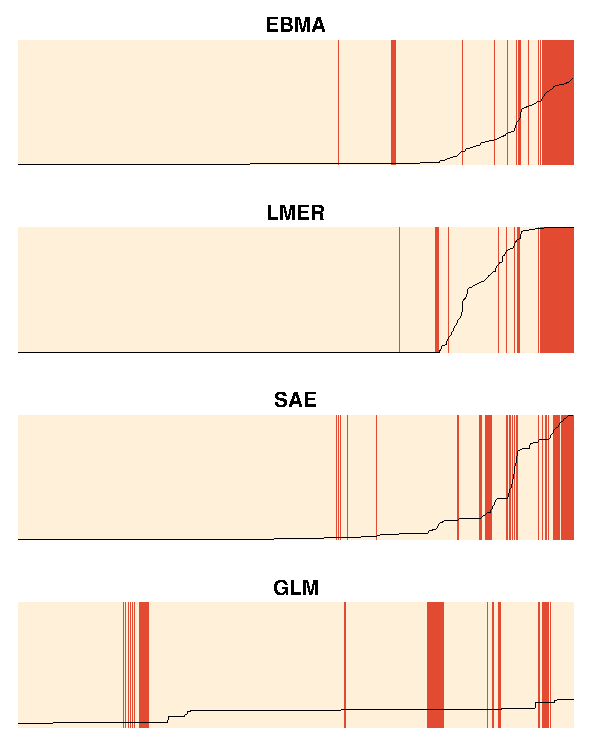
\includegraphics{Insample}
\end{center}
\end{figure}

\begin{figure}
 \caption{\footnotesize Separation plots for the test-period
    predictions of the ICEWS data (n=348).  For each model,
    observations are shown from left to right in order of increasing
    predicted probability (shown as the black line).  Observations
    where insurgency actually occurred are shown in red.  EBMA
    outperforms all component models in assigning high predicted
    probabilities to \textit{more} observed insurgencies and to
    \textit{fewer} non-insurgencies.}
\label{OutSam1sep}
\begin{center}
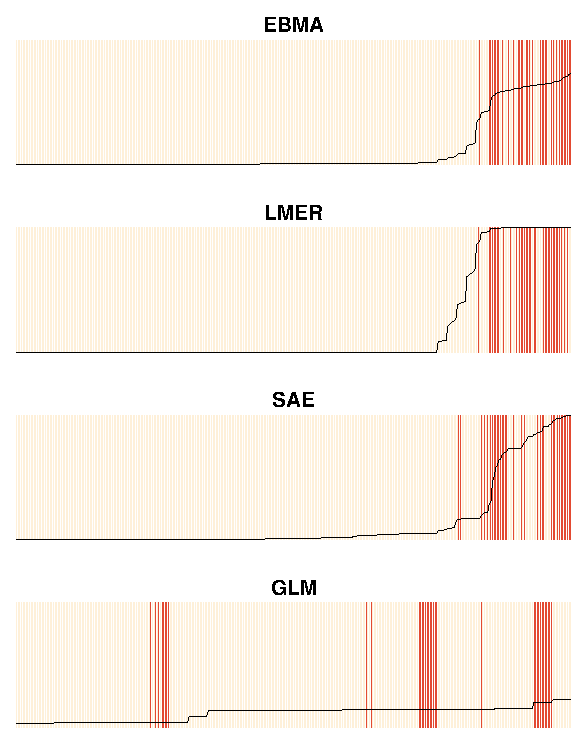
\includegraphics{Outsample}
\end{center}
\end{figure}


 \begin{figure}[p]
   \caption{\footnotesize The predicted and actual percentage of the
     two-party vote going to the incumbent party in U.S. presidential
     elections from six component models and the EBMA forecast.  For
     each year, the plots show the point predictions (circles), 67\%
     predictive intervals (thick horizontal lines), and 90\%
     predictive intervals (thin horizontal lines).  The vertical
     dashed line is the observed outcome.  The EBMA model is
   better calibrated than its components. }
 \label{PresPlots2}
 \begin{center}
 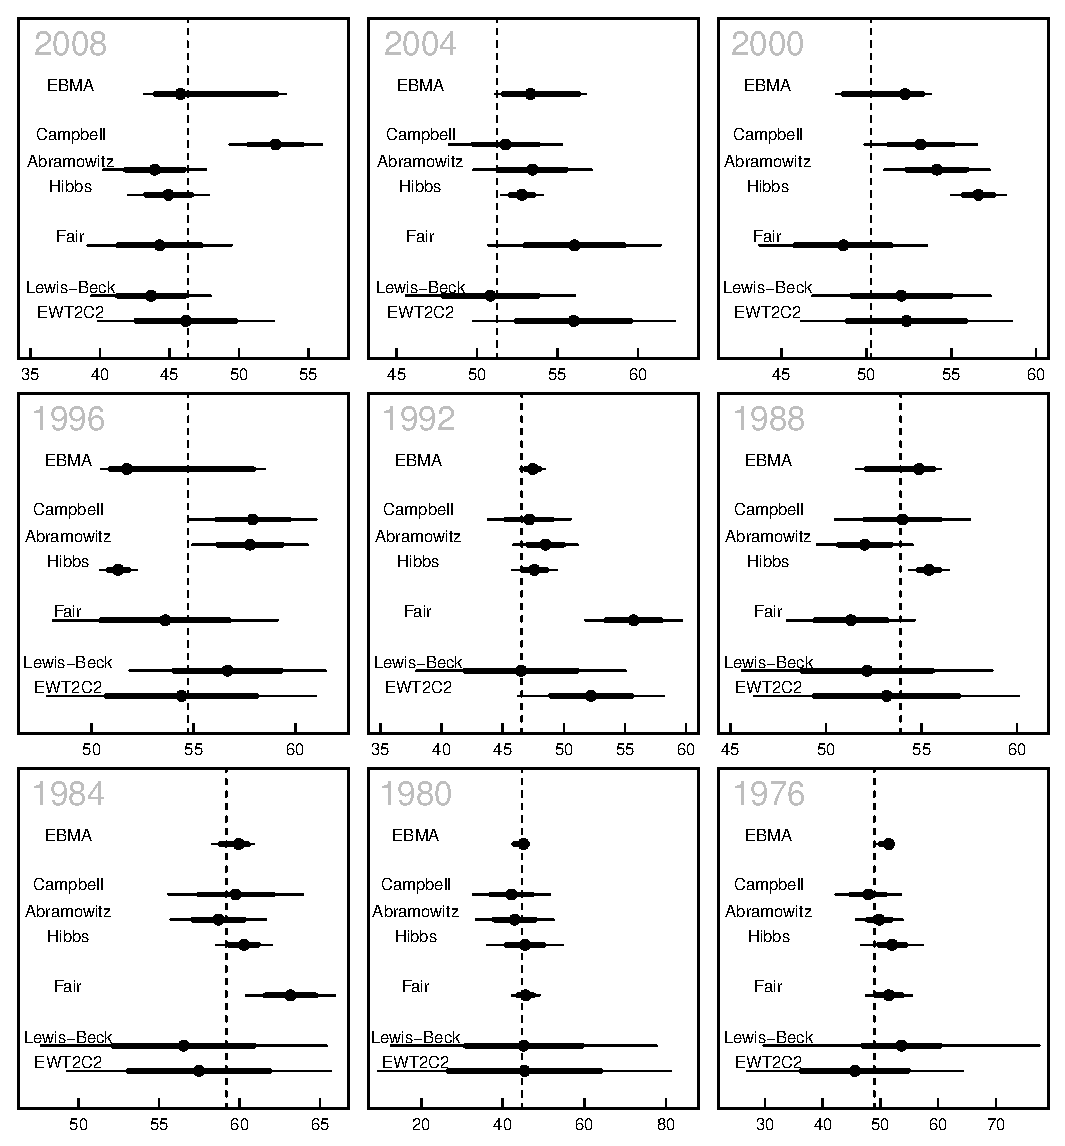
\includegraphics[width=5.6 in]{PresPlot}
 \end{center}
 \end{figure}


\end{document}
\bye
